\subsection{Calling the motion planner}
\label{sec:calling motion planner}

%\begin{figure}[t]
%	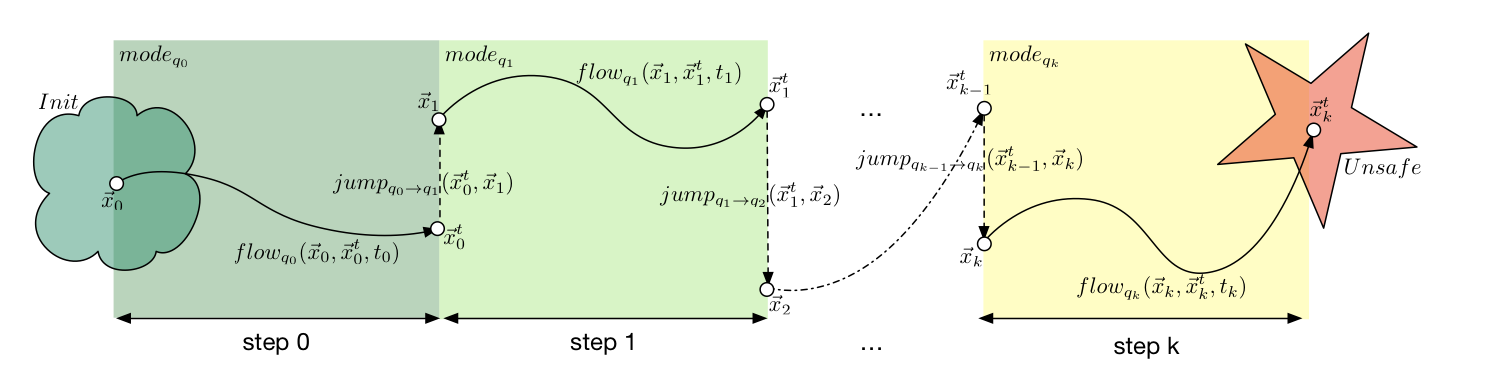
\includegraphics[width=\columnwidth]{figures/unsafe}
%	\caption{The bounded reachability problem in dReach \cite{KongGCC15}}
%	\vspace{-20pt}
%	\label{fig:unsafe}
%\end{figure}

After building the execution tree, APEX starts executing every branch, starting at the root, which is the initial mode $q_0$.
The initial set of continuous states is $X_0$.
A transition is taken if the initial set intersects its guard.
Since $X_0$ may intersect more than one guard, then more than one transition are possible. 
APEX explores all transitions (all branches) in the execution tree.
In each mode APEX enters, $\Bc$ will output a destination $x_B$.
Formally, $x_B$ is a scenario state, but in what remains, it is simpler to think of it as the position that the ego vehicle must reach.

APEX then calls the motion planner to obtain the trajectory that the vehicle will follow.
%See Fig. \ref{fig:apex_internals}.
Since the current state is only known as a set $X_A$, APEX sets the starting point of the trajectory to be the center $x_A$ of $X_A$.
The motion planner then returns a trajectory starting at $x_A$ and ending in a neighborhood of $x_B$.
The neighborhood shape and size are known to APEX and are part of the motion planner's description.
Let that neighborhood be $X_B$. Note that APEX does not place any restrictions on the motion planner's operation and calls it as a black box.
Therefore, the actual motion planner that is used on the real car can be used in the verification of the system.
In this way the verification results are directly applicable to the actual deployed software.